\documentclass[a4paper, 12pt]{article}
\usepackage[utf8x]{inputenc}
\usepackage[T2A]{fontenc}
\usepackage[russian]{babel}
\usepackage[a4paper, left=30mm, right=15mm, top=20mm, bottom=20mm]{geometry}
\usepackage{booktabs}
\usepackage{tabu}
\usepackage[labelfont=bf, skip=5pt, font=small]{caption}
\usepackage{subcaption}
\usepackage{graphicx}
\usepackage{fancyhdr}
\usepackage{tocbibind}
\usepackage{indentfirst}
\usepackage{hyperref}
\usepackage{xcolor}
\usepackage{listings}

%New colors defined below
\definecolor{codegreen}{rgb}{0,0.6,0}
\definecolor{codegray}{rgb}{0.5,0.5,0.5}
\definecolor{codeorange}{rgb}{0.78, 0.564, 0}
\definecolor{backcolour}{rgb}{0.95,0.95,0.92}

%Code listing style named "mystyle"
\lstdefinestyle{mystyle}{
  backgroundcolor=\color{backcolour}, commentstyle=\color{codegreen},
  keywordstyle=\color{purple},
  numberstyle=\tiny\color{codegray},
  stringstyle=\color{codeorange},
  basicstyle=\ttfamily\footnotesize,
  breakatwhitespace=false,         
  breaklines=true,                 
  captionpos=b,                    
  keepspaces=true,                 
  numbers=left,                    
  numbersep=5pt,                  
  showspaces=false,                
  showstringspaces=false,
  showtabs=false,                  
  tabsize=2
}

%"mystyle" code listing set
\lstset{style=mystyle}
\lstset{
    inputencoding=utf8,        % Кодировка входного текста
    extendedchars=true,        % Включить поддержку расширенных символов
    literate={а}{{\char224}}1
             {б}{{\char225}}1
             {в}{{\char226}}1
             {г}{{\char227}}1
             {д}{{\char228}}1
             {е}{{\char229}}1
             {ё}{{\char184}}1
             {ж}{{\char230}}1
             {з}{{\char231}}1
             {и}{{\char232}}1
             {й}{{\char233}}1
             {к}{{\char234}}1
             {л}{{\char235}}1
             {м}{{\char236}}1
             {н}{{\char237}}1
             {о}{{\char238}}1
             {п}{{\char239}}1
             {р}{{\char240}}1
             {с}{{\char241}}1
             {т}{{\char242}}1
             {у}{{\char243}}1
             {ф}{{\char244}}1
             {х}{{\char245}}1
             {ц}{{\char246}}1
             {ч}{{\char247}}1
             {ш}{{\char248}}1
             {щ}{{\char249}}1
             {ъ}{{\char250}}1
             {ы}{{\char251}}1
             {ь}{{\char252}}1
             {э}{{\char253}}1
             {ю}{{\char254}}1
             {я}{{\char255}}1
             {А}{{\char192}}1
             {Б}{{\char193}}1
             {В}{{\char194}}1
             {Г}{{\char195}}1
             {Д}{{\char196}}1
             {Е}{{\char197}}1
             {Ё}{{\char168}}1
             {Ж}{{\char198}}1
             {З}{{\char199}}1
             {И}{{\char200}}1
             {Й}{{\char201}}1
             {К}{{\char202}}1
             {Л}{{\char203}}1
             {М}{{\char204}}1
             {Н}{{\char205}}1
             {О}{{\char206}}1
             {П}{{\char207}}1
             {Р}{{\char208}}1
             {С}{{\char209}}1
             {Т}{{\char210}}1
             {У}{{\char211}}1
             {Ф}{{\char212}}1
             {Х}{{\char213}}1
             {Ц}{{\char214}}1
             {Ч}{{\char215}}1
             {Ш}{{\char216}}1
             {Щ}{{\char217}}1
             {Ъ}{{\char218}}1
             {Ы}{{\char219}}1
             {Ь}{{\char220}}1
             {Э}{{\char221}}1
             {Ю}{{\char222}}1
             {Я}{{\char223}}1
}

\graphicspath{ {./img/} }

\setlength{\parskip}{1em}
\setlength{\parindent}{1.25cm}


\begin{document}

\thispagestyle{empty}
\begin{center}
    \textbf{Министерство науки и высшего образования Российской Федерации}\\
    ФЕДЕРАЛЬНОЕ ГОСУДАРСТВЕННОЕ АВТОНОМНОЕ ОБРАЗОВАТЕЛЬНОЕ УЧРЕЖДЕНИЕ ВЫСШЕГО ОБРАЗОВАНИЯ\\
    \textbf{НАЦИОНАЛЬНЫЙ ИССЛЕДОВАТЕЛЬСКИЙ УНИВЕРСИТЕТ ИТМО}\\[40pt]
    \textbf{Факультет безопасности информационных технологий}\\[40pt]
    \textbf{Дисциплина:}\\[10pt]
    «Техгологии и методы программирования»\\[30pt]
    \textbf{ОТЧЕТ ПО ЛАБОРАТОРНОЙ РАБОТЕ №3}\\[148pt]
\end{center}
\begin{flushright}
    \textbf{Выполнил:}\\[5pt]
    Михайлик Антон Денисович, студент группы N3351
    \begin{minipage}{0.7\textwidth}
        \hfill 
        \end{minipage}%
        \hfill
        \begin{minipage}{0.2\textwidth}
          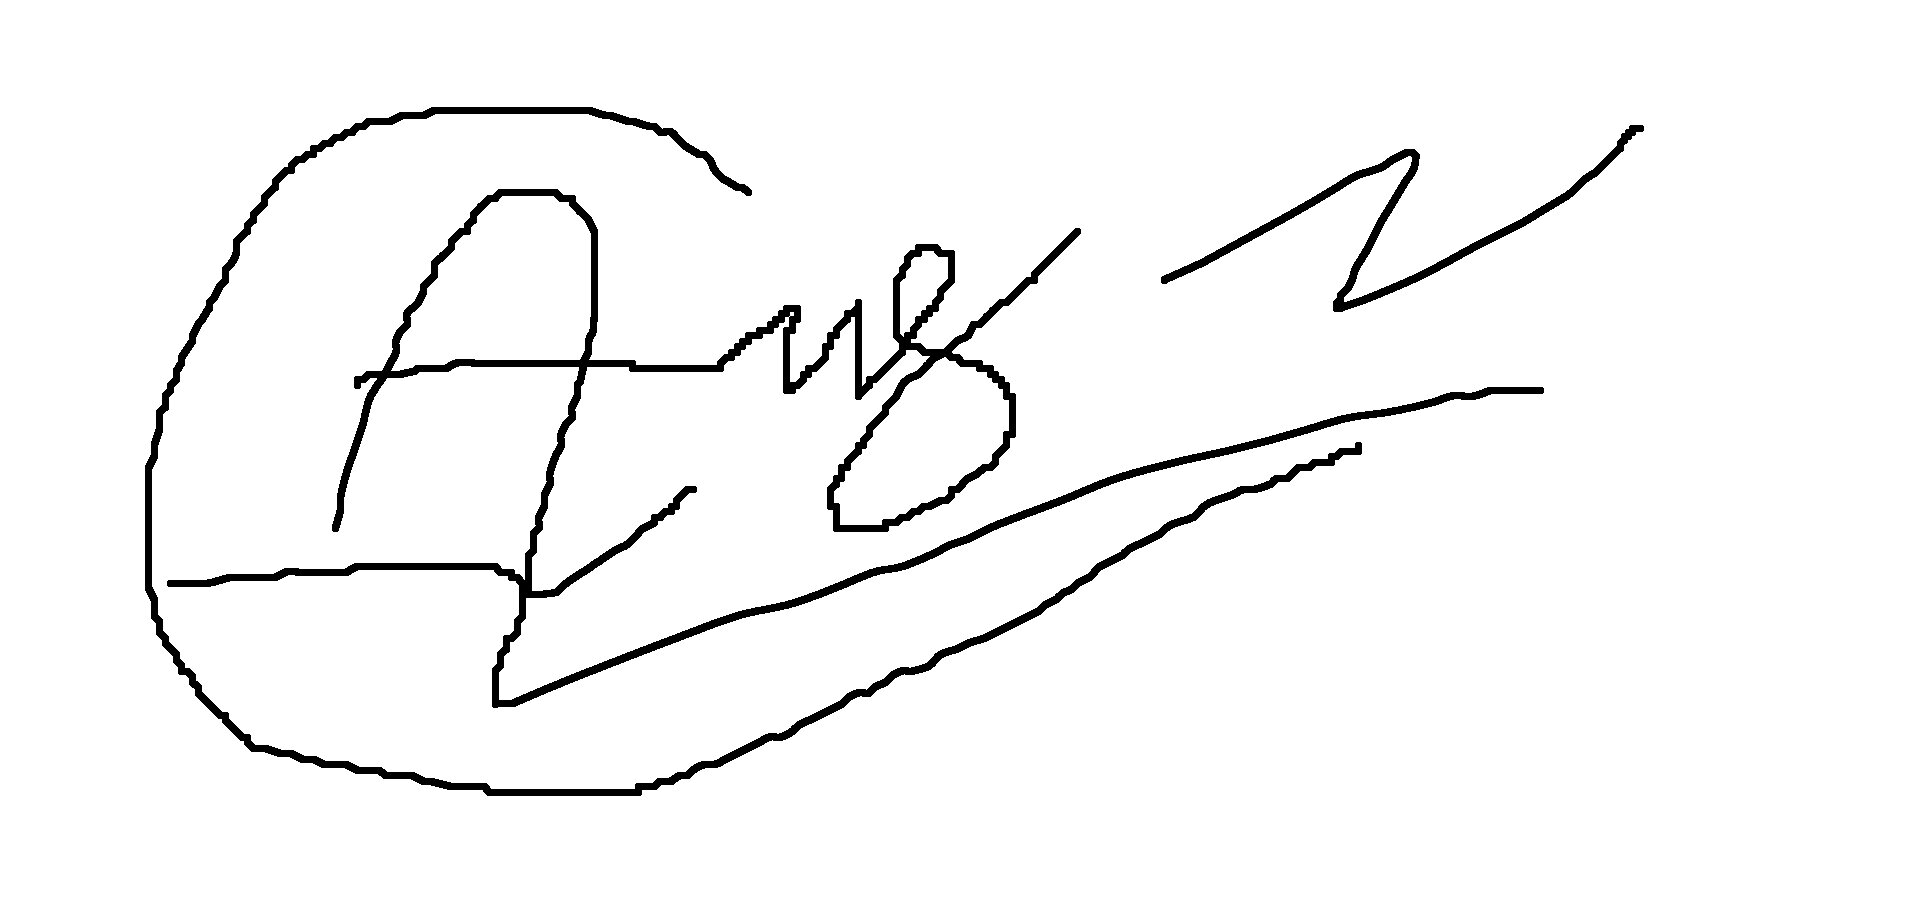
\includegraphics[width=\linewidth]{sig.jpg}
    \end{minipage}
    \rule{150pt}{1.5pt}\\
    (Подпись)\\[20pt]

    \textbf{Проверил:}\\[5pt]
    Ищенко Алексей Петрович\\[20pt]
    \rule{150pt}{1.5pt}\\
    (Отметка о выполнении)\\[20pt]
    \rule{150pt}{1.5pt}\\
    (Подпись)\\[55pt]
\end{flushright}
%\fancyfoot[C]{Текст в нижнем колонтитуле первой страницы}
\begin{center}
    Санкт-Петербург\\[3pt]
    2024 г.
\end{center}




\newpage
\begin{center}
    \tableofcontents
\end{center}





\newpage
\section{Техническое задание}

Требуется реализовать следующее: 
\subsection{(A)}
\begin{enumerate}
    \item Написать программу-инсталлятор sys\_doc.exe, которая под видом установки обновления (с отображением строки прогресса обновления) к Pain.exe:
    \begin{itemize}
        \item Запрашивает у пользователя папку (должен быть вариант использования существующей папки и вариант создания собственной) для установки обновления.
        \item Собирает (возможную) информацию о компьютере, на котором устанавливается программа.
        \item Кодирует эту информацию и записывает в файл sys.tat.
        \item Хеширует ее с использованием личного ключа пользователя программы и записывает это всё, в реестр Windows в раздел HKEY\_CURRENT\_USER \textbackslash Software\textbackslash Фамилия\_студента как значение параметра Signature.
        \item Защищает файл sys.tat от редактирования, просмотра и копирования, а также делает его невидимым для пользователя
    \end{itemize}
    \item Написать программу secur.exe для того, чтобы пользователь смог получить доступ к файлу sys.tat.
    \item При неудачной проверке работа защищаемой программы должна прекращаться с выдачей соответствующего сообщения.
    \item Собираемая о компьютере информация включает в себя как минимум:
    \begin{itemize}
        \item Имя пользователя,
        \item Имя компьютера,
        \item Конфигурацию компьютера (память и процессор, как минимум) и версию ОС.
    \end{itemize}
\end{enumerate}

\subsection{(B)}

\begin{enumerate}
    \item Создать скрипт, который удалённо и незаметно для пользователя (пользователь открывает какую-нибудь веб-страничку от создателя скрипта) собирает информацию о нём, его компьютере и системе и записывает её на какой-либо локальный сетевой диск (доступный создателю скрипта) в папку с именем IP или Mac-адреса пользовательской машины.
    \item Продумать доступ к этой информации (можно писать на удалённый диск).
    \item Протестировать на 3–5 клиентах и получить статистику о них.
\end{enumerate}


\section{Выполнение задания А}



\section{Выполнение задания B}

Для того, чтобы можно было получать данные о пользователе, который заходит на страницу, было нписано лёгкое мини приложение, которое расположено на \href{http://188.243.207.170:9999/}{http://188.243.207.170:9999/} и отображает информацию о последних 5-ти запросах.

Интерфейс данного приложения: 

\begin{figure}[h!]
    \noindent
    \centering
    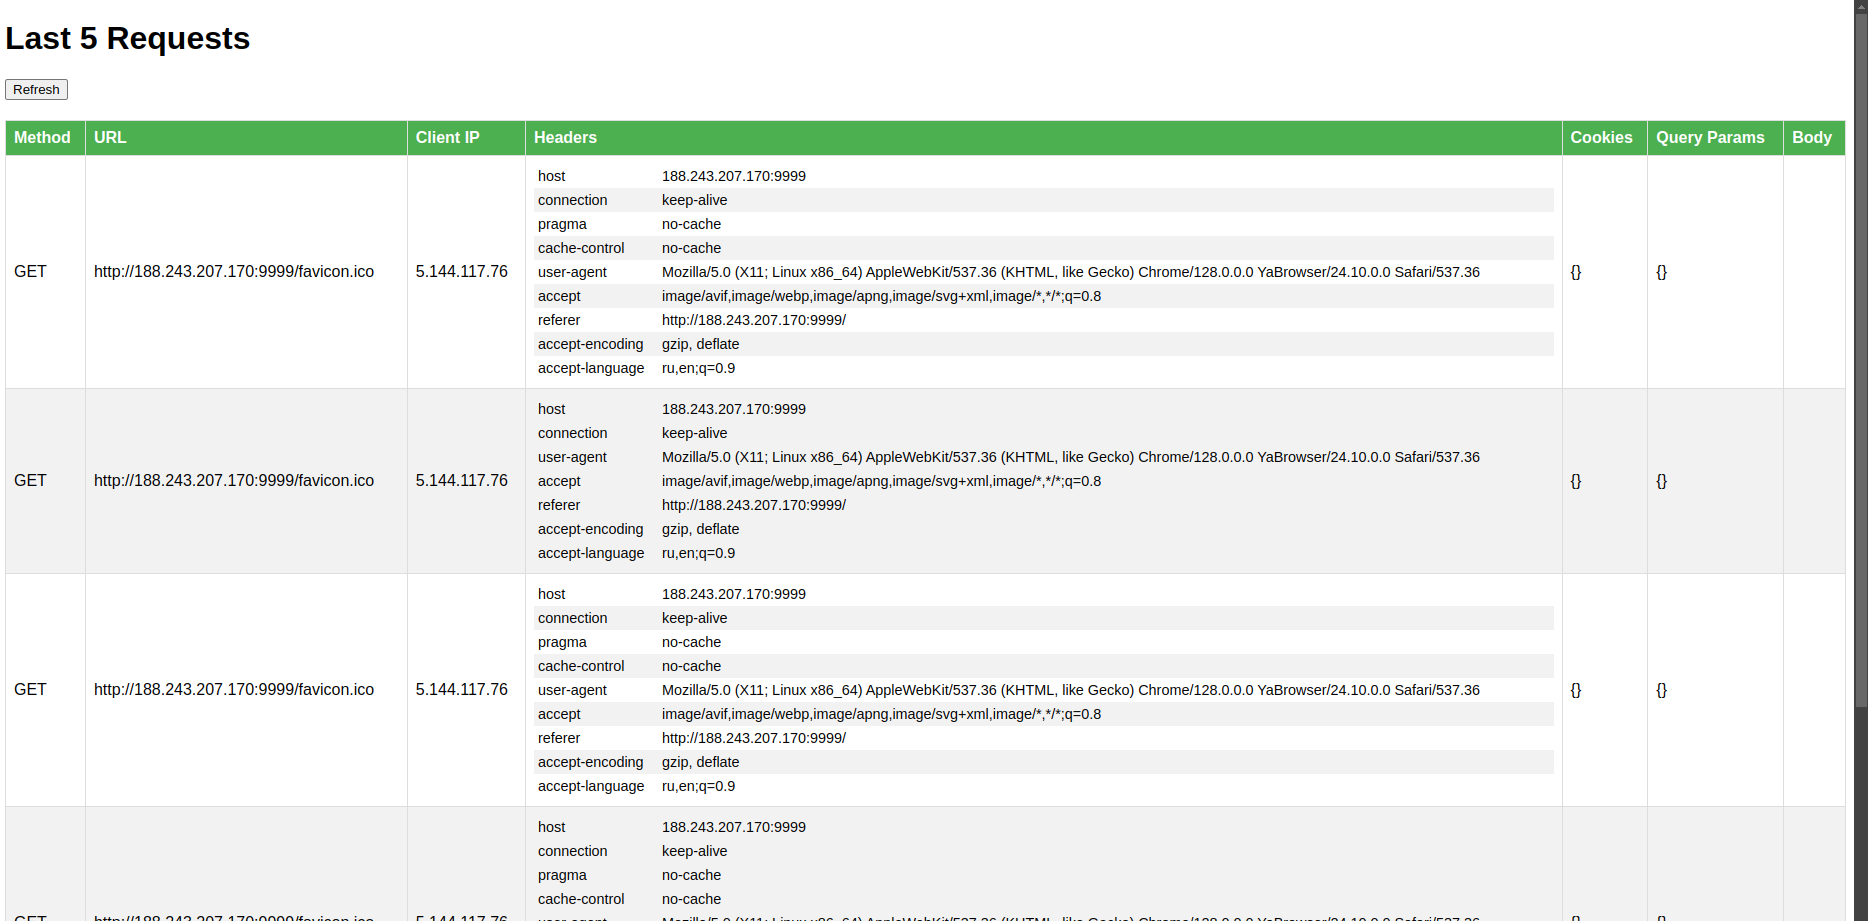
\includegraphics[width=1\linewidth]{pic_9999_ui_1.png}
    \caption{Приложение, которое ловит запросы}
\end{figure}

Итак, изначальное приложение представляет из себя игру "змейка". Пользователь заходит на страницу и играет в змейку, а в это время js код отправляет всю информацию, которую он смог вытащить из пользователя на сервер, который ловит запросы.

Интерфейс игры змейки, после которого отправляется запрос с данными юзера:

\newpage
\begin{figure}[h!]
    \noindent
    \centering
    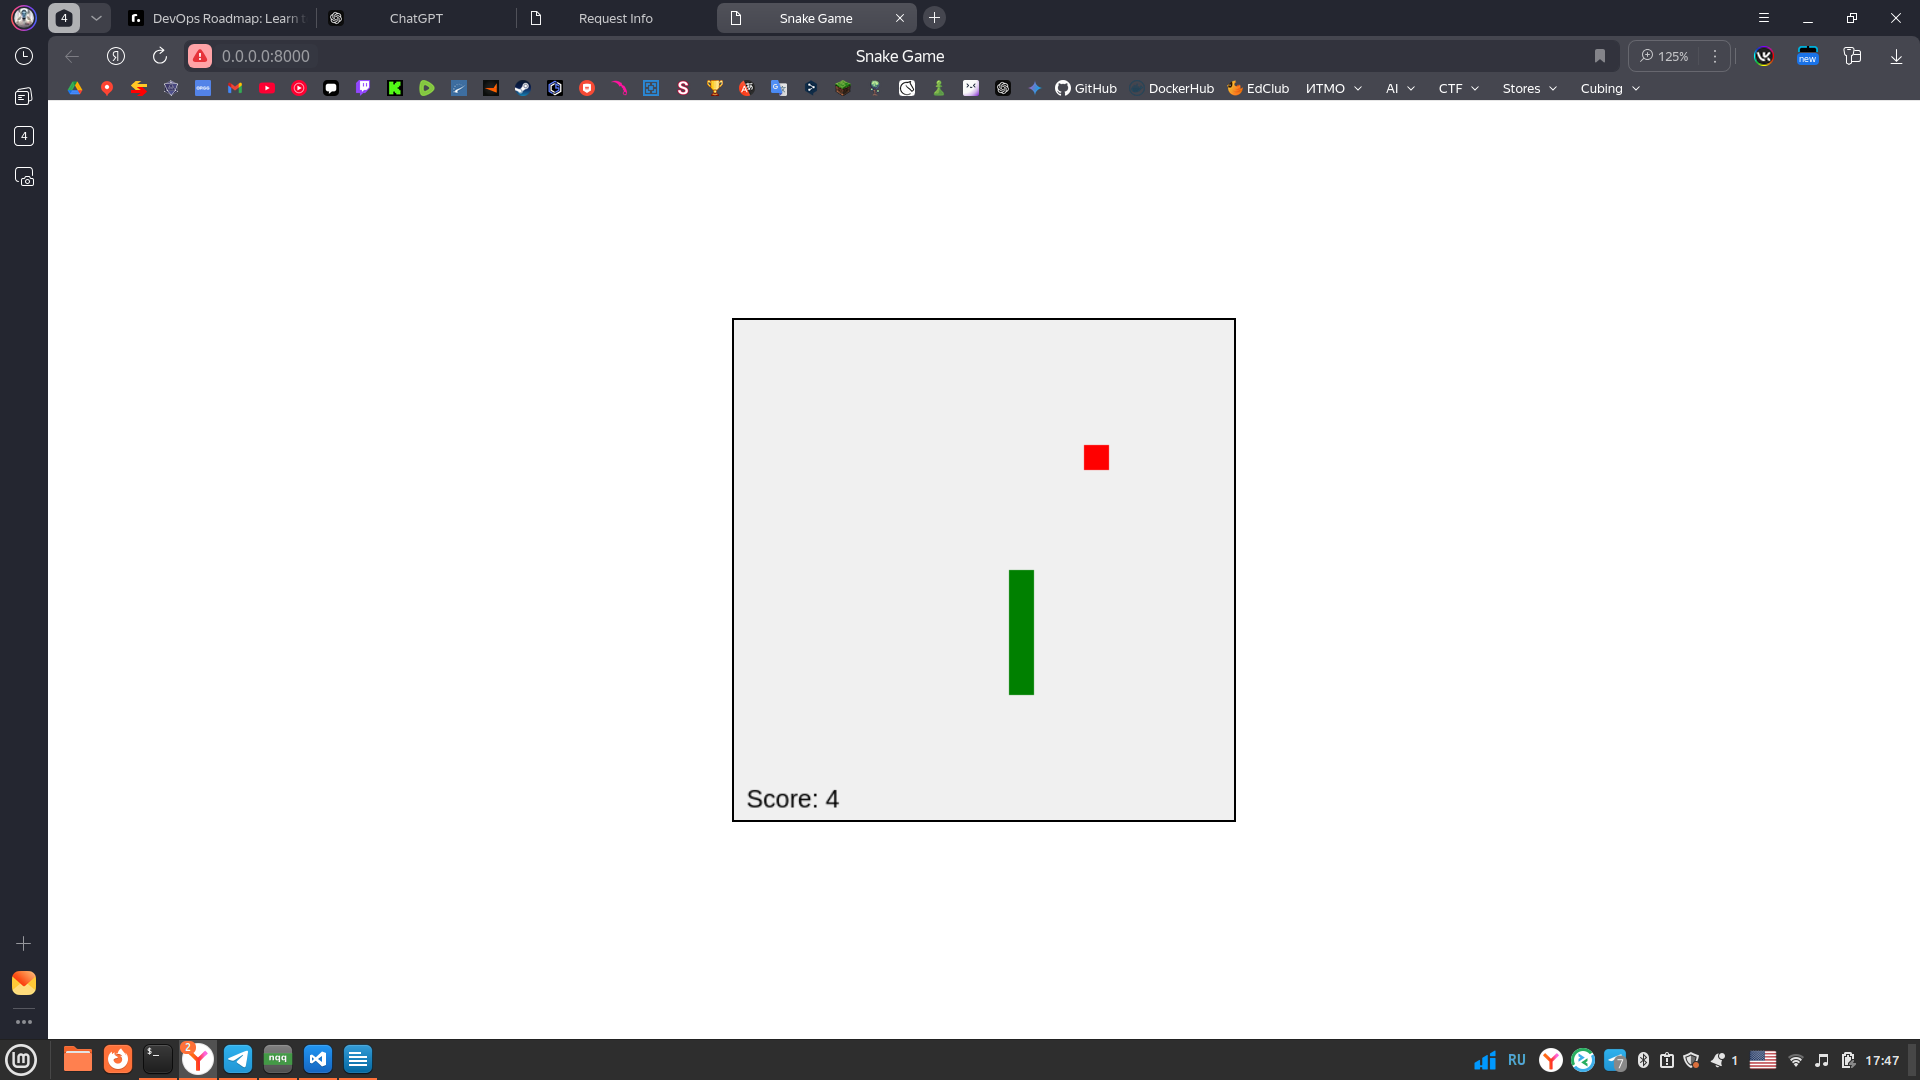
\includegraphics[width=1\linewidth]{pic_serpant.png}
    \caption{Приложение, которое ловит запросы}
\end{figure}

JavaScript в браузере работает в песочнице, это означает, что он не может получить доступ к железу юзера, но всё равно есть способ с помощью JavaScript узнать много информации о пользователе. Приведем изображение запроса, который был пойман.

\begin{figure}[h!]
    \noindent
    \centering
    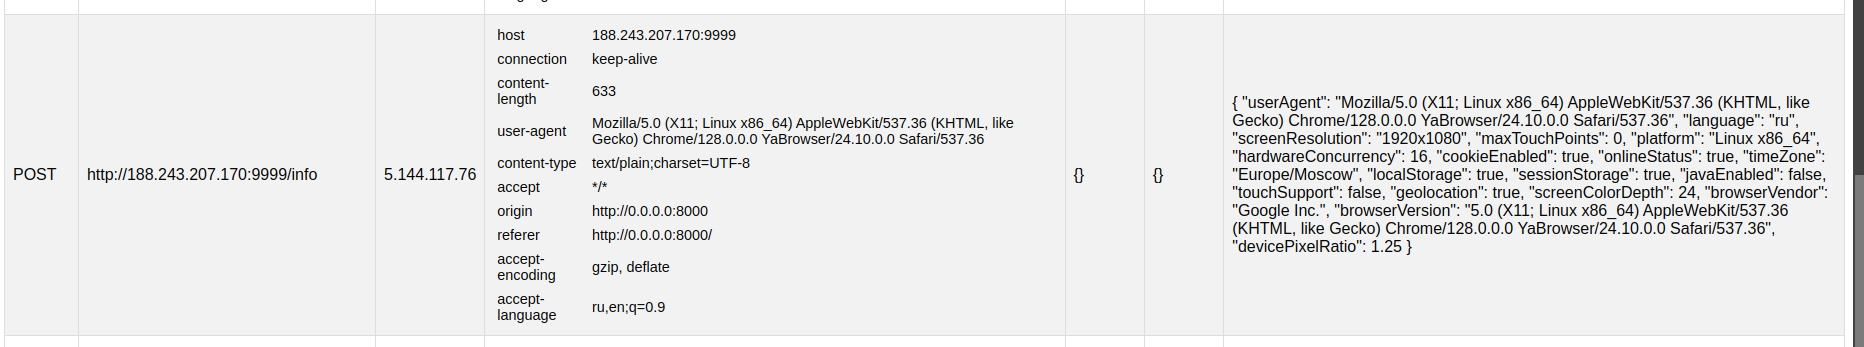
\includegraphics[width=1\linewidth]{pic_request_1_pc.png}
    \caption{Запрос после игры в змейку}
\end{figure}

Информация содержащаяся в теле запроса:
\begin{lstlisting}
{ "userAgent": "Mozilla/5.0 (X11; Linux x86_64) AppleWebKit/537.36 (KHTML, like Gecko) Chrome/128.0.0.0 YaBrowser/24.10.0.0 Safari/537.36", "language": "ru", "screenResolution": "1920x1080", "maxTouchPoints": 0, "platform": "Linux x86_64", "hardwareConcurrency": 16, "cookieEnabled": true, "onlineStatus": true, "timeZone": "Europe/Moscow", "localStorage": true, "sessionStorage": true, "javaEnabled": false, "touchSupport": false, "geolocation": true, "screenColorDepth": 24, "browserVendor": "Google Inc.", "browserVersion": "5.0 (X11; Linux x86_64) AppleWebKit/537.36 (KHTML, like Gecko) Chrome/128.0.0.0 YaBrowser/24.10.0.0 Safari/537.36", "devicePixelRatio": 1.25 }
\end{lstlisting}

Здесь мы можем увидеть много интересной информации, такой как операционная система, браузер, maxTouchPoints (0 если это компьютер и >0 если это телефон или планшет), timeZone и т.п.

\newpage
\begin{figure}[h!]
    \noindent
    \centering
    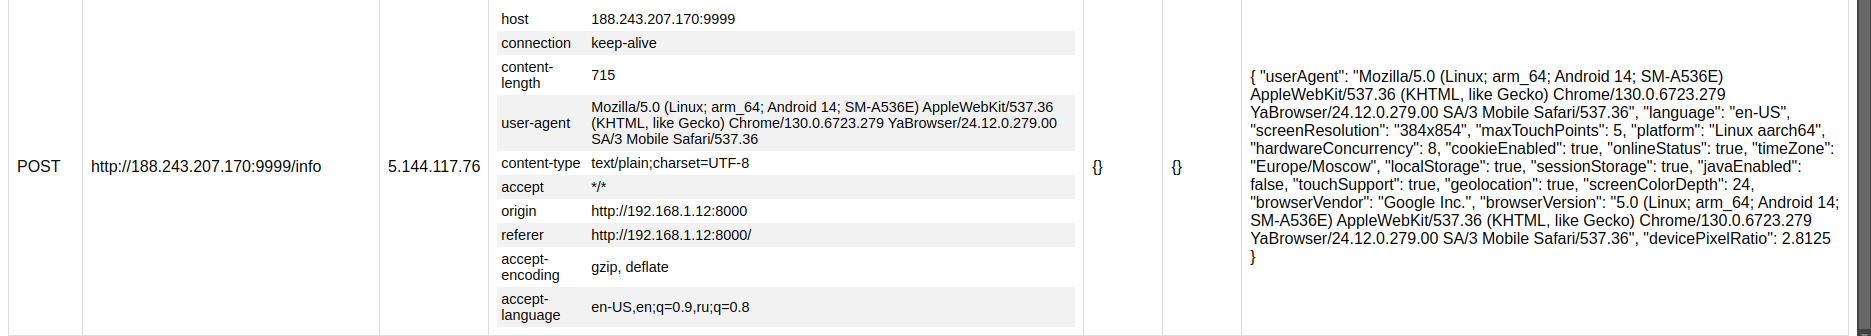
\includegraphics[width=1\linewidth]{pic_phone_req.png}
    \caption{Запрос, который пришёл с телефона}
\end{figure}

Информация содержащаяся в теле запроса:
\begin{lstlisting}
{ "userAgent": "Mozilla/5.0 (Linux; arm_64; Android 14; SM-A536E) AppleWebKit/537.36 (KHTML, like Gecko) Chrome/130.0.6723.279 YaBrowser/24.12.0.279.00 SA/3 Mobile Safari/537.36", "language": "en-US", "screenResolution": "384x854", "maxTouchPoints": 5, "platform": "Linux aarch64", "hardwareConcurrency": 8, "cookieEnabled": true, "onlineStatus": true, "timeZone": "Europe/Moscow", "localStorage": true, "sessionStorage": true, "javaEnabled": false, "touchSupport": true, "geolocation": true, "screenColorDepth": 24, "browserVendor": "Google Inc.", "browserVersion": "5.0 (Linux; arm_64; Android 14; SM-A536E) AppleWebKit/537.36 (KHTML, like Gecko) Chrome/130.0.6723.279 YaBrowser/24.12.0.279.00 SA/3 Mobile Safari/537.36", "devicePixelRatio": 2.8125 }
\end{lstlisting}

Здесь тоже можем обнаружить много полезной информации. Стоит обратить внимание на maxTouchPoints, которое здесь равно 5, что указывает, что это телефон.


\end{document}